% This document provides the style to be used for a MSc Thesis at the
% Parallel and Distributed Systems group
\documentclass[11pt,twoside,a4paper,openright]{report}

% math packages
\usepackage{amsmath}
\usepackage{amssymb}

% textblocks for title page
\usepackage[absolute]{textpos}

% use babel for proper hyphenation
\usepackage[british]{babel}

% Graphics: different for pdflatex or dvi output, choose one
%%\usepackage[dvips]{graphicx}
%%\usepackage[pdftex]{graphicx}
\usepackage{graphicx}

\usepackage{epstopdf}
\usepackage{rotating}
\usepackage{subfigure}

% For nicer tables
\usepackage{booktabs}
\usepackage{tabularx}

% Several sizes for table columns
\newcolumntype{s}{>{\hsize=0.5\hsize}X}
\newcolumntype{t}{>{\hsize=0.25\hsize}X}

% Todo package
\usepackage{todonotes}

% FONT
\usepackage[scaled=.92]{helvet}
%\usepackage{times}

% for url's use "\url{http://www.google.com/}"
\usepackage{url}
\usepackage[plainpages=false]{hyperref} 

% Information that will be filled in at various points in the report
\newcommand{\reportTitle}{TODO TITLE}
\newcommand{\reportAuthor}{B.T. Blokland}
\newcommand{\reportEmail}{b.t.blokland@student.tudelft.nl}
\newcommand{\reportUrlEmail}{\href{mailto:\reportEmail}{\reportEmail}}
\newcommand{\reportMSC}{Embedded Systems} %{Embedded Systems}{Computer Engineering}{Computer Science}{Electrical Engineering}
\newcommand{\reportDate}{\today} %TODO: Dit is de datum van uitgifte van final versie aan de afstudeer commissie 
\newcommand{\presentationDate}{\today} %TODO: Dit is de datum van de afstudeerpresentatie 
\newcommand{\graduationCommittee}{
TODO GRADUATION COMMITTEE & Delft University of Technology \\
TODO GRADUATION COMMITTEE & Delft University of Technology \\
} % The order of listing the names: Graduation prof, supervisor(s), others ordered by title + alphabetical 
%examples: 
%prof. dr. ir. H. J. Sips (chair) & Delft University of Technology \\ 
%ir. dr. D. H. J. Epema           & Delft University of Technology \\ 
\newcommand{\reportAbstract}{TODO ABSTRACT}
\newcommand{\reportKeywords}{TODO KEYWORDS}

% For pdflatex
\pdfinfo{
   /Author (\reportAuthor)
   /Title  (\reportTitle)
   /Keywords (\reportKeywords)
}

\begin{document}

\pagenumbering{alph}
\pagestyle{empty}


% FRONTCOVER
%%\usepackage[total={210mm,297mm},left=0pt,bottom=0pt,top=0cm,right=0pt,headsep=0pt,head=0pt,showframe]{geometry}

%%\input{preambleL31958}
%%\begin{titlepage}
\begin {textblock*}{210mm}(0mm,0mm)
\noindent

\includegraphics[height=3.2cm]{pics/block}
\sffamily
\vspace{.8cm}
\begin{center}
\Large
Delft University of Technology\\
Master's Thesis in \reportMSC\\
\vspace{2cm}
\parbox{170mm}{\bfseries\centering\Huge\reportTitle}\\
\vspace{1cm}
\parbox{170mm}{\bfseries\centering\reportAuthor}

\end{center}
\end{textblock*}

\begin {textblock*}{210mm}[0.0,1.0](0mm,297mm)
\noindent
\hspace{1.89cm}


\hfill\parbox{5cm}{

\includegraphics[width=5cm]{pics/es_logo_cyan_black_rgb}}
\hspace*{2cm}\\

\vspace*{1.5cm}
\noindent

\includegraphics[width=\textwidth]{pics/TU_border_A4_L_front}
\end{textblock*}

\null\newpage


%%%%%%%%%%%%%%%%%%%%%%%%%%%%%%%%%%%%%%%%%%%%%%%%%%%%%%%%%%%%%%%%%%%%%%%%%%%%%%%
\hoffset=1.63cm
\oddsidemargin=0in
\evensidemargin=0in
\textwidth=5in

%%%%%%%%%%%%%%%%%%%%%%%%%%%%%%%%%%%%%%%%%%%%%%%%%%%%%%%%%%%%%%%%%%%%%%%%%%%%%%%
\parindent=1em

% EMPTY PAGE
\cleardoublepage

\pagestyle{plain}
\pagenumbering{roman}
\setcounter{page}{1}

% TITLE PAGE: page i (hidden)
\begin{titlepage}

  \begin{center}
  \null\vfill
    \begin{center}
    \LARGE{\reportTitle}
    \end{center}

    \vspace{3cm}

    \begin{large}
    Master's Thesis in \reportMSC
    \end{large}

    \vspace{1.5cm}

    \begin{normalsize}
    Embedded Software Section\\
    Faculty of Electrical Engineering, Mathematics and Computer Science\\
    Delft University of Technology\\
    Mekelweg 4, 2628 CD Delft, The Netherlands
    \end{normalsize}

    \vspace{2.0cm}

    \begin{normalsize}
    \reportAuthor \\
    \reportUrlEmail
    \end{normalsize}

    \vspace{1.0cm}

    % <MM> DD, YYYY
    \reportDate             %TODO: Dit is de datum van uitgifte van final versie aan de afstudeer commissie

  \vfill
  \end{center}

\end{titlepage}


% GRADUATION DATA AND ABSTRACT: pages ii and iii (hidden)
%De aankondiging bevat de spreker, titel, plaats, datum en tijd, samenstelling van de afstudeercommissie en een korte samenvatting (maximaal 25 regels).
\thispagestyle{empty}

\noindent \textbf{Author}\\
\begin{tabular}{l}
\reportAuthor{} (\reportUrlEmail)\\
\end{tabular}\\
\noindent \textbf{Title}\\
\begin{tabular}{l}
\reportTitle\\
\end{tabular}\\
\noindent \textbf{MSc presentation}\\
\begin{tabular}{l}
% <MM> DD, YYYY (like \today)
\presentationDate\\
\end{tabular}

\vspace{1.1cm}

\noindent \textbf{Graduation Committee}\\
\begin{tabular}{ll}
\graduationCommittee
\end{tabular}


\begin{abstract} %de abstract bevat alleen een korte samenvatting van de inhoud van het onderzoek
\setcounter{page}{3}
\reportAbstract{}
\end{abstract}

\clearpage

%\setcounter{page}{4}

% EMPTY PAGE: page iv
\cleardoublepage

% OPTIONAL QUOTATION: page v
%\pagestyle{empty}

\null\vfill

\begin{center}
\emph{``TODO QUOTE''} -- TODO QUOTED PERSON
\end{center}

\vspace{10cm}

\clearpage


% EMPTY PAGE: page vi
%\cleardoublepage

% PREFACE: page v
\chapter*{Preface}
\addcontentsline{toc}{chapter}{Preface}
TODO MOTIVATION FOR RESEARCH TOPIC

\vspace{1\baselineskip}

\noindent
TODO ACKNOWLEDGEMENTS

\vspace{1\baselineskip}

\noindent
TODO AUTHOR

\vspace{1\baselineskip}

\noindent
Delft, The Netherlands

\noindent
\today

% EMPTY PAGE: page vi
\cleardoublepage

% TABLE OF CONTENTS: starting at page vii
\tableofcontents

\cleardoublepage

\pagenumbering{arabic}
\setcounter{page}{1}

% INTRODUCTION: page 1
\chapter{Introduction}
\label{chp:introduction}

\section{Motivation}
The Internet-of-Things (IoT) is a promising vision which enables billions or trillions of sensor devices to be connected \cite{flicker}. A common bottleneck for such devices is the energy supply. Batteries are large, expensive, heavy and wear out after several years.  %todo add references + note that replacement is an issue

A sustainable solution is energy harvesting where a device collects it's energy from the environment for instance solar, radio frequency (RF), thermal or kinetic energy.

However, developing software for such devices comes with a challenge. Environmental energy can be scarce, causing frequent power failures \cite{tpcthesis}. This contrasts with the standard assumption that programs run continuously throughout execution. The programmer has to take care of this intermittent behavior by for instance storing data to non-volatile memory at certain intervals. The available energy tends to be random, making it difficult to predict how long a program can execute before the next power failure. 

It is hard to conduct repeatable tests due to the random nature of the energy source. While comparing two algorithms, it is impossible to conclude that one algorithm outperforms the other without knowing how much the difference in available energy contributed to the result.

\section{Research goal and contributions}

\textit{Provide a remote accessible testbed to accelerate the development in applications for batteryless devices for those who do not have the resources or tools them selfs and help in finding bugs caused by intermittent behavior.}\\

The proposed architecture of the testbed is shown in Figure \ref{fig:architecture}

Flicker \cite{flicker} would be an ideal platform to use as device under test (DUT), because it supports many software configurable peripherals and has the MSP430 as its core, a common micro controller in low-power applications. An WISP \cite{wisp} could be a possible DUT.

Ekho \cite{ekho} would complement this setup because it can emulate various energy harvesting conditions. An alternative to Ekho would be toggling the power source by a configurable frequency and duty-cycle. Besides emulating, real energy harvesting sources can be used. A configurable light source can be used to power solar panels. An RFID reader can be used to harvest RF energy. 

Several methods can be used to track the progress and outcome of a test: serial console (printf), GPIO tracing (logic analyzer), memory dumping and a debugger (possibly energy aware \cite{edb}).

\begin{figure}[htb]
	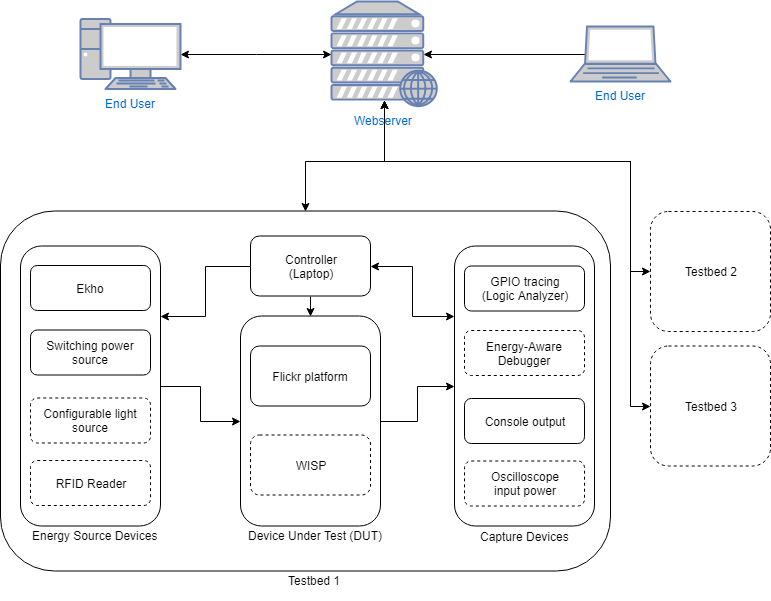
\includegraphics[width=\textwidth]{pics/TestbedArchitecture_v3}
	\caption{Proposed testbed architecture. The dotted lines show optional modules.}
	\label{fig:architecture}
\end{figure}

\section{Thesis outline}

\vspace{1\baselineskip}

\noindent
TODO ORGANISATIONAL DESCRIPTION OF THESIS



\chapter{Related work}
\label{chp:related-work}

The field of energy harvesting devices is promising, but still immature and only a few companies provide such devices commercially. We give an overview of several energy harvesting platforms, both research related and commercial.

Writing software for intermittent devices comes with the challenge of handling frequent and random power cycles. We will discuss which programming models have been developed to counter this issue.

For batteryless, intermittently powered devices there are no publicly available testbeds. Work of \cite{request} enlists properties and features that such a testbed should have, as well as presenting a minimal implementation. The authors call for a more coordinated action in this domain research.

On the other hand there are dozens of existing testbeds for battery-based wireless sensor networks (WSN). There have been many survey published in the past years that compare each of them in detail (see for instance \cite{survey1}, \cite{survey2}). Our goal here is to revise these comparative studies expanding it with the recent developments in testbed deployments.

Besides these testbeds, we will discuss several tools which help in developing applications for batteryless devices.

\section{Energy harvesting platforms}

In this section a brief overview is given of batteryless energy harvesting platforms using various energy sources. This has been surveyed in \cite{sudevalayam2011energy}, \cite{energywsn} ,\cite{talla2015powering} and \cite{kim2014ambient}. Energy harvesting and it's potential with respect to WSNs has been surveyed in \cite{akhtar2015energy} and \cite{bhatti2016energy}.

Table \ref{tab:researchplatforms} shows some popular and recent developed platforms in scientific research. In Table \ref{tab:commercialplatforms} show several companies which are commercially active in the field of energy harvesting devices.

{\renewcommand{\arraystretch}{1.5}
\begin{table*}\footnotesize
\makebox[\linewidth]{ \begin{tabularx}{1.5\textwidth}{sXssssts}
	\toprule
	\textbf{Platform} & \textbf{Description} & \textbf{MCU} & \textbf{Radio} & \textbf{Energy Harvester} & \textbf{Energy Source} & \textbf{Year} & \textbf{Citations}\\
	\midrule

	WISP \cite{wisp} & Family of sensors that are powered and read by UHF RFID readers & MSP430 & \hspace{0pt}Backscattering & Transducer and rectifiers & RF & 2008 & 639 \\
	
	Flexible AD PZT Energy Harvester \cite{aerol} & Self-Powered Wireless Sensor Node Enabled by an Aerosol-Deposited PZT Flexible Energy Harvester & MSP430 & CS2500 & Flexible piezoelectric energy harvester & Kinetic & 2016 & 65\\
	
	Umich Moo \cite{moo} & Improvement on design of WISP & MSP430 & \hspace{0pt}Backscattering & Transducer and rectifiers & RF & 2011 & 63 \\

	Monjolo \cite{monjolo} & Energy-Harvesting AC Power metering which draws zero power under zero load conditions & MSP430 & CC2420 & CR2550, LTC3588 & Power line energy harvesting (magnetic field) & 2013 & 45\\
	
	SPWTS \cite{spwts} & A novel self-powered wireless temperature sensor based on thermoelectric generators & nRF24LE1 & Build in MCU & TEC12706 & Thermal & 2014 & 31\\
	
	Flicker \cite{flicker} & Configurable development board for batteryless IoT & MSP430 & CC1101, nRF51822, backscattering & Solar cell, transducer and rectifiers, LTC3588,  & Solar, RF, Kinetic & 2017 & 11 \\
	
	Capybara \cite{capybara} & Co-designed hardware/software power system with dynamically reconfigurable energy storage capacity & MSP430, CC2650 & CC2650 & TrisolX solar panels, low-power voltage source & Solar, energy source emulation & 2018 & 11 \\
	
	Pible \cite{pible} & BLE batterlyless platform & CC2650 & Build in MCU & Solar panels & Solar & 2018 & 2 \\	
	
	\bottomrule
\end{tabularx}}
\caption{Research Based Energy Harvesting Platforms.}
\label{tab:researchplatforms}
\end{table*}}

{\renewcommand{\arraystretch}{1.5}
\begin{table*}\footnotesize
\makebox[\linewidth]{ \begin{tabularx}{1.5\textwidth}{sXssss}
	
	\toprule
	\textbf{Company} & \textbf{Description} & \textbf{MCU} & \textbf{Radio} & \textbf{Energy Harvester} & \textbf{Energy Source}\\
	\midrule
	
	EnOcean & Various batteryless solutions for i.e.Building Automation and Smart Home & 8051 processor & TCM 3x0 & ECO 200, ECS 300, ECT 310 Perpetuum & Solar, motion, thermal\\

	Powercast & Provides wireless power solutions, RFID tags, RF power transmitter,  RF power harvester & PIC24F & IEEE 802.15.4 transceiver, TX91502 & PCC110 & RF\\
	
	Williot & Makes a batteryless bluetooth beacon device based on RF harvesting & ARM processor & N/A & N/A & RF\\
	
	PsiKick & Provides batteryless monitoring solutions to mainly the industry. Related to the university of Virginia and Michigan. & Custom ULP SoC, ARM architecture \cite{customsoc} & Build in SoC & N/A & Solar, thermal\\
	
	Bellutech & BelluTech’s patented batteryless wireless miniature sensors continuously track and record exposure to environmental and operating conditions. & N/A & N/A & N/A & RF\\	
	
	Matrix Industries & Makes a batteryless thermoelectric powered smartwatch & N/A & N/A & N/A & Thermal\\

	\bottomrule
\end{tabularx}}
\caption{Commercial Energy Harvesting Platforms.}
\label{tab:commercialplatforms}
\end{table*}}


\section{Programming Models For Intermittent Computing}
\begin{figure}[htb]
	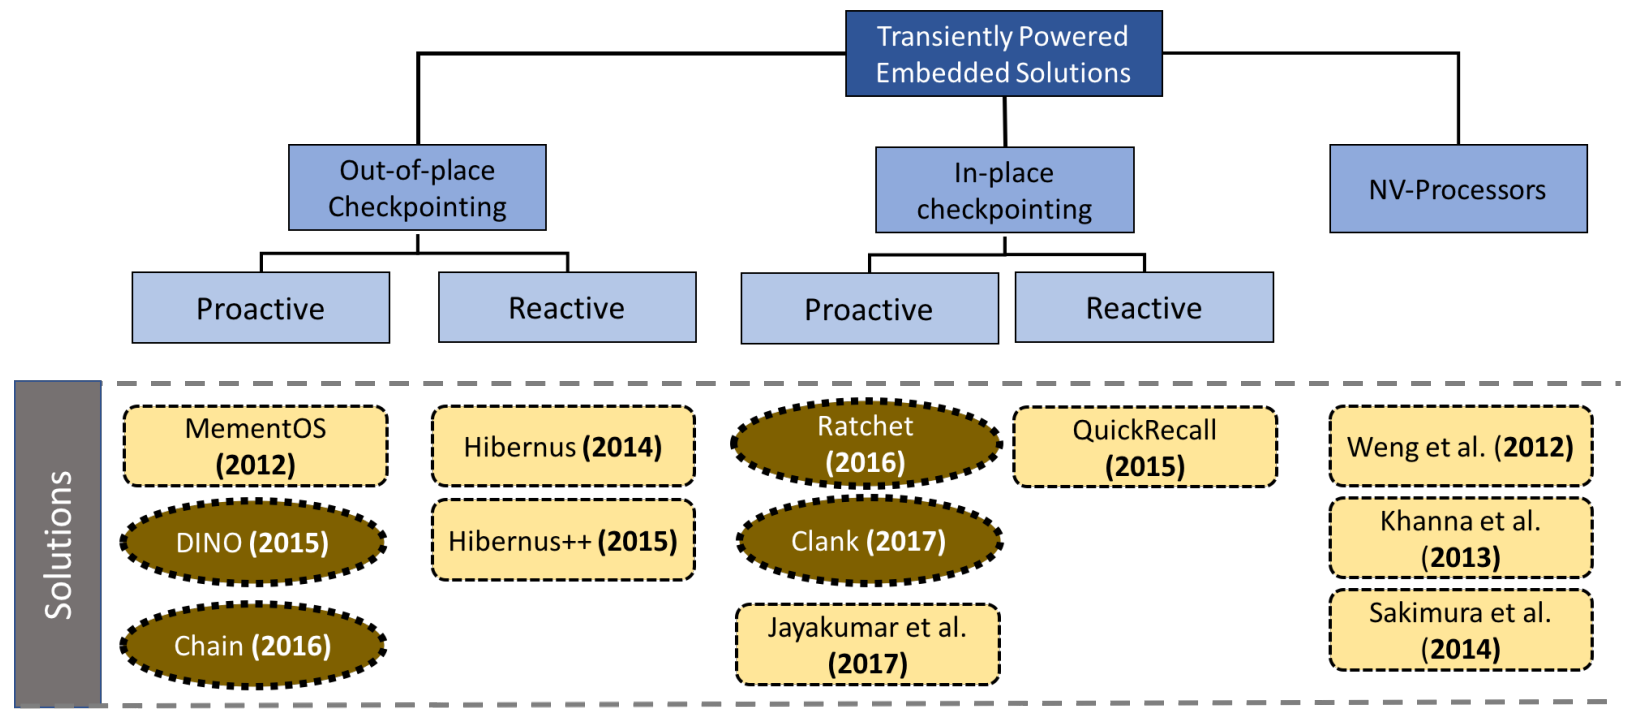
\includegraphics[width=\textwidth]{pics/taxonomy-tpc}
	\caption{Taxonomy of several programming models for intermittent computing \cite{tpcthesis}.}
	\label{fig:architecture}
\end{figure}


\section{Wireless Sensor Network Testbeds}
\label{sec:wireless-sensor-networks}
\todo{Paraphrase this section, taken from https://www.iotbench.ethz.ch/}

\subsection{FIT IoT-LAB}
FIT IoT-LAB \cite{FIT-IoT} provides a very large scale infrastructure facility suitable for testing small wireless sensor devices and heterogeneous communicating objects.

IoT-LAB features over 2000 wireless sensor nodes spread across six different sites in France.  Nodes are either fixed or mobile and can be allocated in various topologies throughout all sites.  A variety of wireless sensors are available, with different processor architectures (MSP430, STM32 and Cortex-A8) and different wireless chips (802.15.4 PHY @ 800 MHz or 2.4 GHz).  In addition, “open nodes” can receive custom wireless sensors for inclusion in IoT-LAB testbed.

\subsection{Flocklab}

Flocklab \cite{flocklab} is a wireless sensor network (WSN) testbed, developed and run by the ​Computer Engineering and Networks Laboratory at the ​Swiss Federal Institute of Technology Zurich (ETH Zurich) in Switzerland. FlockLab's key features include:
\begin{itemize}
	\item FlockLab's observer based testbed architecture which provides services for detailed testing of sensor nodes:
	\item Time accurate pin tracing
	\item Time accurate pin actuation
	\item Power measurements
	\item Serial interface logging and writing
	\item Voltage control to simulate e.g. battery depletion
\end{itemize}

\subsection{Indriya2}

Indriya2 \cite{indriya2} is a three-dimensional wireless sensor network deployed across three floors of the School of Computing , at the National University of Singapore (NUS). The Testbed facilitates research in sensor network programming environments, communication protocols, system design, and applications. It provides a public, permanent framework for development and testing of sensor network protocols and applications. Users can interact with the Testbed through an intuitive web-based interface designed based on Harvard's Motelab's interface. Registered users can upload executables, associate those executables with motes to create a job, and schedule the job to be run on Testbed. During the job execution, all messages and other data are logged to a database which is presented to the user upon job completion and then can be used for processing and visualization. 

\section{Development Tools For Batteryless Devices}

\todo{Make this section more technical, provide a table comparing tools and add introductory paragraph}

\subsection{Ekho}

To counter the issue of randomness in a energy harvesting power source, Ekho \cite{ekho} has been developed. This an emulator capable of accurately recreating harvesting conditions in a lab. It reproduces the I-V characteristics of energy harvesting sources, allowing developers to choose from a library of energy traces recorded with various sources and environmental conditions.

\subsection{Flicker}
\todo{Paraphrase this section}
Flicker \cite{flicker} is a platform for quickly prototyping batteryless embedded sensors. Flicker is an extensible, modular, “plug and play” architecture that supports RFID, solar, and kinetic energy harvesting; passive and active wireless communication; and a wide range of sensors through common peripheral and harvester interconnects. Flicker supports recent advances in failure-tolerant timekeeping, testing, and debugging, while providing dynamic federated energy storage where peripheral priorities and user tasks can be adjusted without hardware changes.

\subsection{Energy aware debugger}
\todo{Paraphrase this section}
The Energy-Interference-Free Debugger (EDB) \cite{edb}, is a tool for monitoring and debugging of intermittent systems without adversely affecting their energy state. EDB recreates a familiar debugging environment for intermittent software and augments it with debugging primitives for effective diagnosis of intermittence bugs.





% Example chapters
% CHAPTERS ... For instance: History/Prior Work, Design/Implementation, Experiments
%\chapter{CHAPTER TITLE}
\label{chp:CHAPTERTITLE}
INTRODUCTION TEXT TO THIS CHAPTER IN WHICH ALL SECTIONS ARE DESCRIBED ROUGHLY (1 SENTENCE EACH).

This chapter describes the ... In Section~\ref{sec:SECTIONTITLE}, examples are given of how to use tables and figures in MSc theses.

\section{SECTION TITLE}
\label{sec:SECTIONTITLE}

Every caption of a table (or figure) should start with a capital letter, and should end with a period. References to tables are given with a capital letter for table, as in ``(see Table~\ref{tab:EXAMPLETABLE})'' or ``in Table~\ref{tab:EXAMPLETABLE}, ...''.

\begin{table}[htb]
\centering
\begin{tabular}{|l|c|r|}
\hline % horizontal line
left aligned & centred & right aligned \\
\hline \hline
12           & 34      & 56            \\
\hline
\end{tabular}
\caption{Complete sentence describing the tabular data.}
\label{tab:EXAMPLETABLE}
\end{table}

References to figures are given with a capital letter for figure, as in ``(see Figure~\ref{fig:EXAMPLEFIGURE})'' or ``in Figure~\ref{fig:EXAMPLEFIGURE}, ...''.

\cite{b}
\cite{a}

\begin{figure}[htb]
% most GNUplot figures need to be rotated, width should be the same throughout the complete document, and no extension is needed

\includegraphics[angle=180,width=\textwidth]{pics/TUD_logo_zw}
\caption{Complete sentence describing the figure thoroughly.}
\label{fig:EXAMPLEFIGURE}
\end{figure}


% CONCLUSIONS AND FUTURE WORK
%\chapter{Conclusions and Future Work}
\label{chp:conclusionsandfuturework}

\section{Conclusions}
TODO CONCLUSIONS

\section{Future Work}
TODO FUTURE WORK



% BIBLIOGRAPHY
%#define SORTED 1
\bibliographystyle{bib/latex8}
\bibliography{bib/mycollection}

%\appendix

%\chapter{TODO APPENDIX NAME}
\label{app:}
Appendix body



\end{document}

